\chapter{Parte 6}
\label{c:parte6}

\vspace{1cm}

\newpage

\section{Speeded-up Robust Features (SURF)}
  % SURF (Speeded-UP Robust Features) es un detector y descriptor invariante a escala y rotación. El mismo, posee buenas propiedades de repetibilidad, distintividad y robustez permitiendo además calcularse y ser comparado relativamente rápido respecto a otros métodos como por ejemplo SIFT.
  % La tarea de buscar puntos correspondientes entre dos imágenes de la misma escena u objeto es parte de muchas aplicaciones de visión computacional entre las cuales podemos mencionar, la registración de imágenes (transformar conjuntos de datos en coordenadas), calibración de la cámara, reconocimiento de objetos, restauración de imágenes, entre otras.
  % 
  % La búsqueda de correspondencias de puntos discretos de imagen pude ser dividida en tres pasos. Primeramente, se seleccionan ``puntos de interés'' que vienen dados por posiciones distintivas de la imagen como esquinas, uniones tipo T, puntos que difieren de su vecindad respecto a color o brillo, etc. La propiedad mas valorada de un detector de puntos de interés es su repetibilidad, la cual expresa la confianza del detector en encontrar los mismos puntos de interés físicos bajo diferentes condiciones de visualización. Luego, la vecindad de cada punto de interés es representada por un vector de características el cual debería ser distintivo, robusto al ruido, detección de desplazamientos, deformaciones geométricas y fotométricas (idealmente). Finalmente, se buscan las coincidencias entre los vectores descriptores de las diferentes imágenes. Esta búsqueda se encuentra basada en la distancia entre los vectores (por ejemplo la distancia mahalanobis o la euclídea). Aquí se debe hacer notar que la dimensión del descriptor tiene un impacto directo en el tiempo de computo. Así, dimensiones pequeñas resultan deseables para correspondencias rápidas, sin embargo, por lo general vectores de este tipo resultan menos distintivos que su contra parte los de alta dimensiones.

  % Es nuestro objetivo desarrollar un detector y descriptor que en comparación con el estado del arte sea más rápido de calcular sin sacrificar su rendimiento. Con el objetivo de tener éxito en la tarea, se debe encontrar un balance entre ambos requerimientos como simplificar el esquema de detección mientras se mantiene la precisión, y reducir el tamaño del descriptor mientras se mantiene suficientemente su distintividad.

  Una gran variedad de detectores y descriptores han sido propuestos en la literatura (ej. 21,24,27,37,39,25).
  También, comparaciones y evaluaciones de rendimiento sobre los conjuntos de datos han sido estudiadas (28,30,31).

  % Nos enfocaremos en un detector y descriptor invariante a la escala y a la rotación en el plano. Tanto el detector como el descriptor no utilizan información de color, sino que se valen de una imagen en escala de grises para llevar a cabo el procedimiento. Estos, parecen ofrecer un buen compromiso entre la complejidad de las características y la robustez a las deformaciones que comúnmente ocurren. La distorsión o torcimiento, escalado anisotrópico\footnote{En geometría euclídea, el \textbf{Escalado uniforme} o \textbf{Escalado isotrópico} es una transformación lineal que incrementa o decrementa un objeto por un factor de escala el cual es el mismo en todas las direcciones. El resultado del escalado, es similar (en sentido geométrico) al original. Si se utiliza al menos un factor de escala diferente para un eje de coordenadas, se está en presencia de un \textbf{Escalado no uniforme} o \textbf{Escalado Anisotrópico} resultando en un cambio en la forma del objeto.} y efectos de la perspectiva se asumen que son alteraciones de segundo orden que son cubiertos en cierto grado por la robustez general del descriptor. %Note que el descriptor puede ser extendido hacia regiones invariantes afines\footnote{Una transformación afín entre dos espacios vectoriales (estrictamente hablando, dos espacios afines) consiste en una transformación lineal seguida de una traslación. En general una transformación afín está compuesta de transformaciones lineales (rotaciones, homotecias y sesgos) compuestas con una traslación o desplazamiento} usando la normalización afín de la elipse (31), aunque esto tendrá un impacto sobre el tiempo de cálculo. %Extendiendo el detector, por otro lado, es menos directo. En cuanto a las deformaciones fotométricas se supone un modelo lineal con un desplazamiento (sesgo) y un cambio de contraste (factor de escala). 

  En la sección \ref{sec:seccion3}, se describirá la estrategia aplicada para la detección rápida y robusta de los puntos de interés. La imagen de entrada es analizada a diferentes escalas con el objetivo de garantizar invariancia a cambios de escala. Los puntos de interés detectados son provistos con un descriptor invariante a escala y rotación en la sección \ref{sec:seccion4}. Además, se propone una técnica simple y sencilla de indexación, basada en el contrate del punto de interés con su vecindad.

  En la sección \ref{sec:seccion5}, algunos de los parámetros disponibles y sus efectos son discutidos, incluyendo los beneficios de la versión no invariante a la rotación (U-SURF o Up right SURF). También se investiga la aplicación de surf a dos importantes escenarios de aplicación. Primero, se considera el caso especial de registración de imágenes sobre la calibración de la cámara para reconstrucción 3d. Luego, se exploran las aplicaciones de SURF a un experimento de reconocimiento de objetos. Ambas aplicaciones muestran los beneficios de SURF en términos de velocidad y robustez a diferencia de otras estrategias.

\subsection{Trabajos relacionados}
  \subsubsection{Detección de puntos de interés}
  

  \subsubsection{Descripción de puntos de interés}
  Una larga variedad de descriptores de características han sido propuestos tales como las derivadas del gaussiano (11), momentos invariantes (32), características complejas (1,36), filtros orientables (12), características locales basadas en la fase (6), y descriptores representando la distribución de características de escalas más pequeñas dentro del vecindario del punto de interés. Mas tarde, introducido por Lowe(24), mostró que supero a los otros(28). Esto puede explicarse por el hecho de que capturo una cantidad de información sustancial sobre patrones espaciales de intensidad, mientras que al mismo tiempo era robusto a deformaciones pequeñas y errores de localización. 

  Varios refinamientos en este esquema básico han sido propuestos. Ke y Sukthankar (18) aplicaron PCA en la imagen gradiente alrededor del punto de interes detectado. Este método PCA-SIFT construye un descriptor de 36 dimensiones que es más rápido para buscar coincidecnias, pero es menos distintivo que SIFT de acuerdo al estudio de Mikolajczyk (30);  y aplicar PCA hace más lento el cálculo de características. En la misma publicación (30), los autores propusieron una variante a SIFT, llamada GLOH, que resultó ser más distintiva con el mismo numero de dimensiones. Sin embargo GLOH es computacionalmente más caro ya que utiliza también PCA para la compresión de los datos.

  El descriptor SIFT parecía permanecer como el descriptor más adecuado para usos prácticos y por lo tanto el más usado en estos días. Es distintivo y relativamente rápido lo que es crucial para aplicaciones on line. Recientemente Se y otros (37) implementaron SIFT en una FPGA (Field Programmable GAte Array) y mejoraron su velocidad en un orden de magnitud. Mientras tanto, Grabner y otros (14) también han usado imágenes integrales para aproximar SIFT. Su paso de detección se basa en la diferencia de la media (sin interpolación), y la descripción en histogramas integrales. Alcanzaron aproximadamente la misma velocidad (aunque el paso de descripción es constante en la velocidad), pero a cambio de reducir la calidad comparado con SIFT. Generalmente, dimensiones altas del descriptor es una desventaja de SIFT en el paso de correspondencias. Para aplicaciones on-line que recaen sobre una PC común, cada uno de los tres pasos (detección, descripción y correspondencia), deberían ser rápidos.

  Un cuerpo extenso de trabajos hay disponible con el objetivo de mejorar la velocidad en el paso de correspondencias. Todos ellos vienen a expensas de obtener una aproximación a la correspondencia exacta. Se pueden mencionar best-bin-first propuesto por Low(24), balltress(35), vocabulary trees (34), locality sensitive hashing(9) o redundan bit vectores(13). Complementariamente a esto, nosotros sugerimos usar la traza de la matriz hessiana para incrementar la velocidad de correspondencia. Junto con las dimensión baja de los descriptores, cualquier algoritmo de coincidencias debe realizar la tarea más rápidamente.

\subsection{Detección de puntos de interés}
\label{sec:seccion3}
% La detección de puntos de interés propuesta por SURF, usa una aproximación básica a la matriz Hessiana que junto con el uso de imágenes integrales \ref{Viola01rapidobject} y combinado con los filtros caja (boxlets \ref{Simard99boxlets:a}) permiten reducir el tiempo de cálculo de forma considerable.
% 
% \subsubsection{Imágenes integrales}
% Las imágenes integrales, permiten calcular más rápidamente la convolución con filtros caja. La imagen de entrada $\mathit{I_{\sum}(x)}$ en la posición $\mathbf{x}=(x,y)^{T}$ representa la suma de todos los píxeles de la imagen de entrada $\mathit{I}$ dentro de una región rectangular formada por el origen y $\mathbf{x}$.
% 
% Una imagen integral $I_{\sum}(x,y)$ es una imagen en la que el valor del píxel $p=(x,y)$ es la suma de todos los valores de los píxeles entre $p$ y el origen, expresado por la ecuación \ref{eq:integral_image_1}
% 
% \begin{equation}
%  \label{eq:integral_image_1}
% \mathit{I}_{\sum}(x,y)=\sum_{i=0}^{i\leq x}\quad\sum_{j=0}^{j\leq y}I(i,j)
% \end{equation}
% 
% Una vez que la imagen integral se ha calculado, son necesarias tres sumas para calcular la suma de las intensidades sobre cualquier área rectangular vertical (ver figura \ref{fig:integral_image_sum}). El tiempo de cálculo resulta independiente del tamaño lo cual favorece en la aproximación de SURF en la que se utilizan filtros de grandes tamaños. 
% 
% \begin{figure}[tbhp]
%    \centering
%         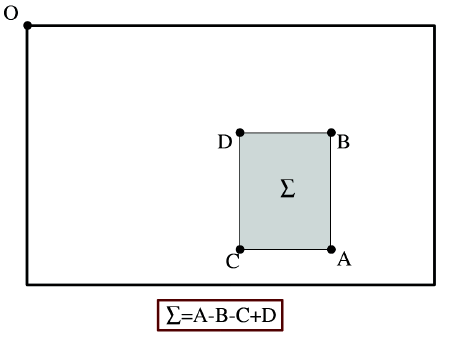
\includegraphics[scale=0.4]{./figs/sumintegralimages}
%     \caption[Suma de intensidades en un rectángulo usando imágenes integrales]{Usando imágenes integrales, solo toma tres adiciones y cuatro operaciones de acceso a memoria para calcular la suma de las intensidades dentro de una la región rectangular independientemente de su tamaño}
%    \label{fig:integral_image_sum}                %% Etiqueta para la figura entera
% \end{figure}

\subsubsection{Puntos de interés basados en la Matriz Hessiana}
% El detector SURF se encuentra basado en la matriz hessiana ya que la misma posee buen rendimiento y logra buena precisión en sus resultados. Tanto para la selección de escala como para la determinación de la ubicación de puntos o regiones (se establecen cuando se da un máximo), se lleva a cabo mediante el determinante del Hessiano.
% 
% Dado un punto $\mathbf{x}=(x,y)$ en la imagen $\mathit{I}$, la matriz Hessiana $\mathcal{H}(\mathbf{x}, \sigma)$ en $\mathbf{x}$ en la escala $\sigma$ viene definida como:
% \begin{equation}
% \mathcal{H}(\mathbf{x},\sigma)=\left[\begin{array}{cc}
% \mathit{L_{xx}(\mathbf{x},}\sigma)\hphantom{} & \mathit{L_{xy}(\mathbf{x},}\sigma)\\
% \mathit{L_{xy}(\mathbf{x},}\sigma)\hphantom{} & \mathit{L_{yy}(\mathbf{x},}\sigma)
% \end{array}\right],
% \end{equation}
% donde $\mathit{L_{xx}(\mathbf{x},}\sigma)$ es la convolución de la derivada gaussiana segunda $\frac{\partial^{2}}{\partial x^{2}}\mathit{g}(\sigma)$ con la imagen $\mathit{I}$ en el punto $\mathbf{x}$ y similarmente para $\mathit{L_{xy}(\mathbf{x},}\sigma)$ y $\mathit{L_{yy}(\mathbf{x},}\sigma)$

Si bien los gaussianos son óptimos para el análisis espacio-escala \ref{Koenderink84, Lindeberg90scale-spacefor}, en la práctica necesitan ser discretizados y truncados (Ver Fig. \ref{fig:gaussiansapproximationskernels} izquierda), resultando esto en una una pérdida de repetibilidad bajo rotaciones de imágenes cercanas a múltiples impares de $\frac{\pi}{4}$, debilidad que se cumple en general para detectores basados en el Hessiano. Sin embargo, los detectores siguen teniendo un buen desempeño y la ligera disminución en el rendimiento no superan la ventaja de las convoluciones rápidas alcanzadas por la discretización y el truncado. %Además, como los filtros reales no son ideales, en cualquier caso 
% y dado el éxito de Lowe con sus aproximaciones LoG, hemos llevado la 
Así, se aproxima a la matriz hessiana con filtros caja \footnote{Filtro caja: es un filtro promediador simple: promedio de todos los píxeles en una región dada} (ver Fig. \ref{fig:gaussiansapproximationskernels} derecha), los cuales aproximan las derivadas gaussianas de segundo orden y pueden ser evaluados con un costo computacional bajo usando las imágenes integrales, resultando en tiempos de cálculo independientes del tamaño del filtro utilizado.
% . Como se muestra en la sección de resultados y en la figura \ref{fig:graphrendimiento}, el rendimiento es igual o mejor que con los gaussianos discretos y recortados.
Notar que debido a la forma cuadrada de estos filtros, la repetibilidad alcanza un máximo en múltiplos de $\frac{\pi}{2}$.

% La figura \ref{fig:graphrendimiento} muestra la tasa de repetibilidad de dos detectores basados en la matriz del hessiano en una imagen con un cambio rotacional puro. La repetibilidad alcanza un máximo alrededor de múltiplos de $\frac{\pi}{2}$. Esto es debido a la forma cuadrada del filtro. 
\begin{figure}[tbhp]
   \centering
        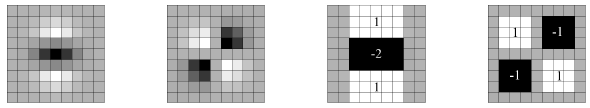
\includegraphics[scale=0.4]{./figs/gaussiansapproximationskernels}
    \caption[Kernels gaussianos aproximados y discretizados]{De izquierda a derecha: Las derivadas parciales de segundo orden gaussianas (discretas y truncadas) en la dirección $\mathit{y-}\hphantom{}(\mathit{L}_{yy})$ y $\mathit{xy}\hphantom{}(\mathit{L}_{xy})$ respectivamente; aproximaciones para las derivadas parciales de segundo orden gaussianas en las direcciones $\mathit{y-}\hphantom{}(\mathit{D}_{yy})$ y $\mathit{xy}\hphantom{}(\mathit{D}_{xy})$. Las regiones grises son iguales a cero.}
   \label{fig:gaussiansapproximationskernels}                %% Etiqueta para la figura entera
\end{figure}

Los filtros caja de 9x9 de la figura \ref{fig:gaussiansapproximationskernels} corresponden a aproximaciones de un gaussiano con $\sigma=1.2$ y representan la escala más baja (resolución espacial más alta) para el cálculo del mapa de respuestas de regiones y puntos que difieren en sus propiedades de intensidad o color comparado con su vecindad. Denotando las mismas con $\mathit{D}_{xx}$, $\mathit{D}_{yy}$ y $\mathit{D}_{xy}$, produce que el determinante del Hessiano venga definido por \ref{eq:deth}
\begin{equation}
\label{eq:deth}
\det(\mathcal{H}_{approx})=D_{xx}D_{yy}-(wD_{xy})^{2} 
\end{equation}

% %%begin de 3:
% Aquí, $D_{xx}$ es el filtro caja aproximado de $L_{xx}(\mathbf{x},\sigma)$
% %%end de 3

La ponderación relativa $w$ de la respuesta del filtro es usada para balancear la expresión del determinante Hessiano. Si bien el mismo varía para diferentes escalas, en la práctica se puede establecer al factor constante $w=0.9$, ya el  mismo no tiene un impacto significante en los resultados de acuerdo a los experimentos. %Esto es necesario por la conservación de la energía entre los kernels gaussianos y sus aproximados,

% \begin{equation}
% w=\frac{|L_{xy}(1.2)|_{F}|D_{yy}(9)|_{F}}{|L_{yy}(1.2)|_{F}|D_{xy}(9)|_{F}}=0.912\ldots\simeq0.9
% \end{equation}

% donde $|x|_{F}$ es la norma de Frobenius. Note que para que sea teóricamente correcto, los cambios de ponderaciones dependen de la escala. 
% DEn la práctica, mantendremos este factor constante, ya que el mismo no tiene un impacto significante en los esultados de acuerdo a los experimentos.

% Las respuestas de los filtros son normalizadas con respecto a su tamaño. Esto garantiza una norma de Frobenius constante para cualquier tamaño de filtro lo cual es un importante aspecto para el análisis escala espacio que se discutirá en la próxima sección.

La aproximación al determinante del Hessiano, representa las respuestas de regiones y puntos que difieren de su vecindad en la posición $\mathbf{x}$. Esta respuestas son guardadas en un mapa de respuestas sobre diferentes escalas y máximos locales son detectados como se explica en la sección \ref{sec:sec34}.
% 
% \begin{figure}[tbhp]
%    \centering
%         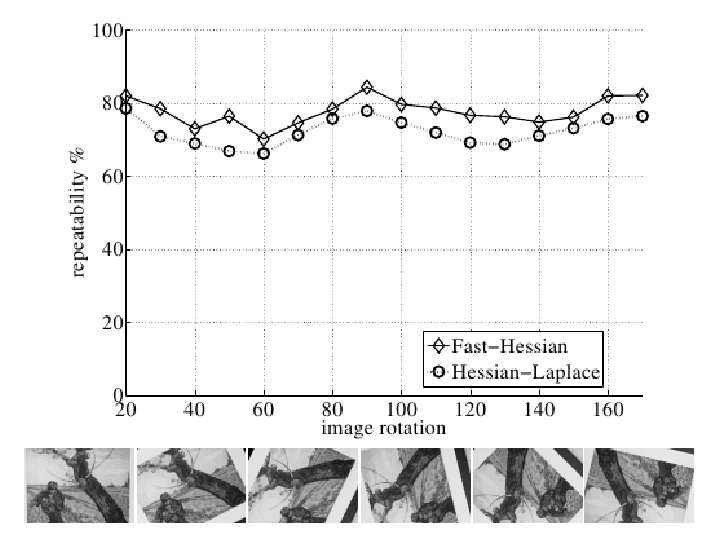
\includegraphics[scale=0.4]{./figs/graphrendimiento}
%     \caption[]{Arriba: Repetibilidad para una imágen rotada hasta 180 grados. Los detectores basados en el Hessiando, en general tienen repetibilidad menor para ángulos múltiplos impares de $\frac{\pi}{4}$. Abajo: Imágenes de ejemplo usadas. El Fast-Hessian es la versión más precisa de nuestro detector (FG-15), como se expondrá en la sección \ref{sec:section33}}
%    \label{fig:graphrendimiento}                %% Etiqueta para la figura entera
% \end{figure}

\subsubsection{Representación Espacio Escala}
\label{sec:section33}
Los puntos de interés necesitan ser encontrados en diferentes escalas, entre otras cosas porque la búsqueda de correspondencias a menudo requiere la comparación de imágenes que han sido vistas en diferentes escalas. Los espacios escala usualmente son implementadas como una pirámide de imágenes. Las imágenes son suavizadas repetidamente mediante un filtro gaussiano y luego son sub muestreadas con el objetivo de alcanzar un nivel mayor en la pirámide. Lowe \ref{Lowe:2004:DIF:993451.996342} restó las capas de la pirámide para obtener las imágenes DoG (diferencia de gaussianos) donde los regiones y puntos de interés pueden ser encontrados.

Gracias al uso de los filtros caja y las imágenes integrales, no se necesita aplicar iterativamente el mismo filtro a la salida de la capa previamente filtrada, sino que se puede aplicar filtros caja de cualquier tamaño a la misma velocidad directamente sobre la imagen original e incluso de forma paralela %(pero esto no es explotado aquí).
Por lo tanto, el espacio escala es analizado mediante el incremento del tamaño del filtro en vez de reducir iterativamente el tamaño de la imagen, ver Fig. \ref{fig:pyramidfilters}. La salida del filtro de 9x9 introducido en la sección anterior, es considerada la capa de la escala inicial, cuyo valor $s=1.2$ (aproximación de la derivada gaussiana con $\sigma=1.2$). Las capas siguientes son obtenidas mediante el filtrado de la imagen con máscaras cada vez mas grandes, teniendo en cuenta la naturaleza discreta de imágenes integrales y la estructura específica de los filtros.

La principal motivación para este tipo de muestreo es la eficiencia computacional. Además, como no se sub muestrea la imagen, no hay aliasing. La desventaja es que los filtros cajas preservan las componentes de alta frecuencia que pueden perderse al tomar la escena más alejada, lo cual limita la invarianza a escala. Sin embargo, esto no fue notable en los experimentos realizados en la implementación original según lo afirma el autor.

\begin{figure}[tbhp]
   \centering
        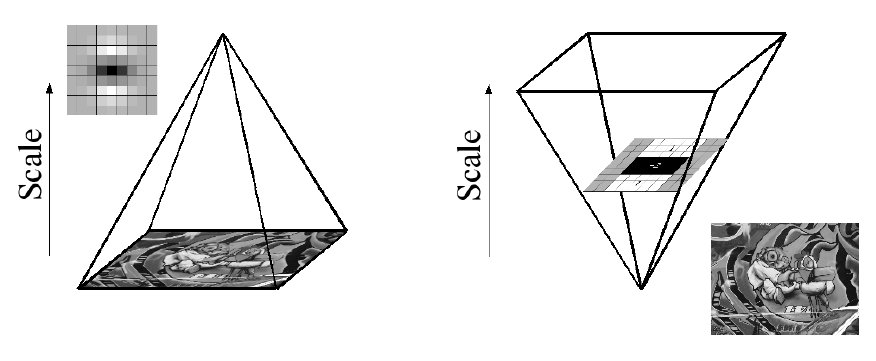
\includegraphics[scale=0.4]{./figs/pyramidfilters}
    \caption[Pirámide de imágenes]{En vez de reducir iterativamente el tamaño de la imagen (izquierda), el uso de las imágenes integrales permiten aumentar el tamaño del filtro a un costo constante (derecha).}
   \label{fig:pyramidfilters}          %% Etiqueta para la figura entera
\end{figure}

El espacio escala es divido en octavas. Una octava representa una serie de mapas de respuesta del filtro obtenida por convolución de la misma imagen con un filtro cuyo tamaño se va incrementando. En total, una octava comprende un factor de escala de 2 (lo que implica que se necesita más de el doble del tamaño del filtro como se verá mas abajo). Cada octava es subdividida en un número constante de niveles de escala. Debido a la naturaleza de las imágenes integrales, la mínima diferencia de escala entre dos escalas subsecuentes depende de la longitud $l_0$ del lóbulo positivo o negativo de la derivada parcial de segundo orden en la dirección de derivación ($\mathit{x}$) o ($\mathit{y}$), que se establece en un tercio del tamaño del filtro. Para un filtro de 9x9, esta longitud $l_{0}$ es 3. Para dos niveles sucesivos, se incrementa el tamaño por un mínimo de 2 píxeles (un píxel por cada lado) con el objetivo de mantener el tamaño impar para asegurar la presencia de un píxel central. Esto resulta en un incremento total del tamaño de la máscara por 6 píxeles (ver figura \ref{fig:filterincrementsize}. Note que para dimensiones diferentes de $l_{0}$ (por ejemplo el ancho de la banda central del filtro vertical de la figura \ref{fig:filterincrementsize}), re-escalar la máscara introduce errores de redondeo. Sin embargo, dado que estos errores comúnmente son muchos menores que $l_{0}$, esta aproximación resulta aceptable.
\begin{figure}[tbhp]
   \centering
        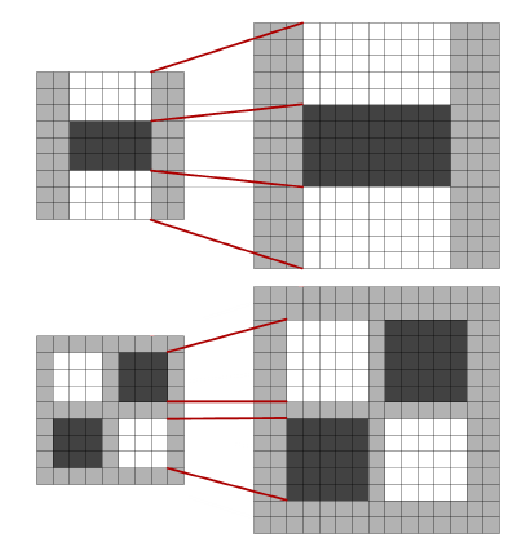
\includegraphics[scale=0.4]{./figs/filterincrementsize}
    \caption[]{Filtros $\mathit{D}_{yy}$ (arriba) y $\mathit{D}_{xy}$ (abajo) para dos niveles de escalas sucesivas (9x9 y 15x15). La longitud del lóbulo oscuro solo puede ser incrementado por un número de píxeles par con el objetivo de garantizar la presencia de un píxel central (arriba) }
   \label{fig:filterincrementsize}                %% Etiqueta para la figura entera
\end{figure}

La construcción de la dimensión escala empieza con filtros de 9x9, que calculan la regiones y puntos de interés de la imagen para la escala más pequeña. Luego, filtros con tamaño 15x15, 21x21 y 27x27 son aplicados, por lo que se alcanza a superar la duplicación de la escala por 2. Pero esto es necesario ya que la supresión de los no máximos en 3D ha sido aplicada tanto espacialmente y sobre las escalas vecinas. Luego, el primer y último mapa de respuestas hessianas de la pila no puede contener estos máximos, que han sido usados por razones de comparación únicamente. Por lo tanto, después de la interpolación \ref{sec34}, la escala posible más pequeña es $\sigma=1.6=1.2\frac{12}{9}$ correspondiente a un filtro de tamaño 12x12, y la más grande es $\sigma=3.2=1.2\frac{24}{9}$.
Para más detalles referirse a 2.

Consideraciones similares se tienen para otras octavas. Para cada nueva octava, el tamaño del filtro es incrementado por 2 (yendo de 6 a 12, 12 a 24, 24 a 48). Al mismo tiempo, los intervalos de muestreo para la extracción de puntos de interés se duplican así como se hacia con cada nueva octava. Esto reduce el tiempo de computo y la perdida de precisión es comparable al que sucede con el sub muestreo en imágenes en las aproximaciones tradicionales. Los tamaños de los filtros para la segunda octava son 15, 27, 39 y 51. Para la tercera se calcula con tamaños de 27, 51, 75, 90 y si la imagen original es más grande que el tamaño de  los filtros correspondientes, el análisis espacio escala se aplica sobre una cuarta escala, usando filtros de tamaño 51, 99, 147 y 195. La figura \ref{fig:tamfilters} da un paneo del tamaño de los filtros para las primeras 3 octavas. Se debe aclarar que cuando más octavas son analizadas, el número de puntos detectados por octavas decae rápidamente, como se puede apreciar en la figura \ref{fig:histogramoctaves}.
\begin{figure}[tbhp]
   \centering
        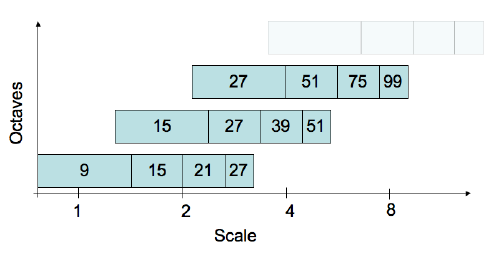
\includegraphics[scale=0.4]{./figs/tamfilters}
    \caption[Representación gráfica de las longitudes de los filtros para 3 diferentes octavas]{Representación gráfica de las longitudes de los filtros para 3 diferentes octavas. El eje logarítmico horizontal representa las escalas. Observar que las octavas están solapadas con el objetivo de cubrir todas las posibles escalas.}
   \label{fig:tamfilters}               %% Etiqueta para la figura entera
\end{figure}

\begin{figure}[tbhp]
   \centering
        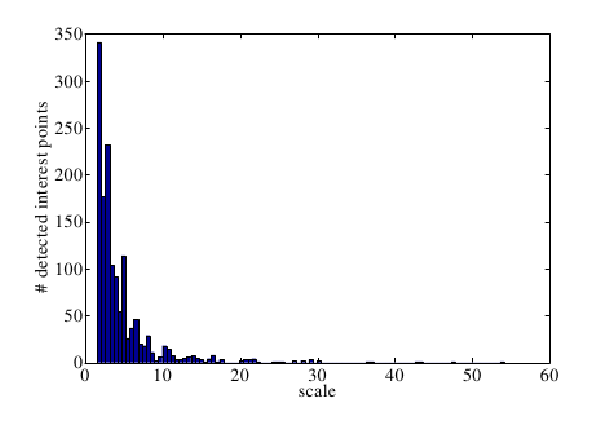
\includegraphics[scale=0.4]{./figs/histogramoctaves}
    \caption[Histogramas de las escalas detectadas]{Histogramas de las escalas detectadas. El número de puntos de interés por octava decae rápidamente}
   \label{fig:histogramoctaves}                %% Etiqueta para la figura entera
\end{figure}

Los cambios de grandes escalas, especialmente entre los primeros filtros y las octavas (9 a 15 es un cambio de 1.7), representa las muestras de escalas algo toscas. Por lo tanto, también hemos implementado un espacio escala con un muestreo de escalas mas fino. Esta primero duplica el tamaño de la imagen, usando interpolación lineal, y luego empieza la primer octava mediante el filtrado con un filtro de tamaño 15. Los filtros adicionales son 12,27,33 y 39. Luego se inicia una segunda octava, usando filtros que se incrementan en 12 píxeles su tamaño, después de lo cual sigue una tercera y cuarta octava. Ahora el cambio de escala entre los dos primeros filtros es solo $1.4 (21/25)$. La escala más pequeña para la versión más precisa que se puede detectar a través de interpolación cuadrática es $s=(1.2\frac{18}{9})/2=1.2$.

Como la norma de Frobenius se mantiene constante para los filtros de cualquier tamaño, la escala esta normalizada y no se requiere ponderación para las respuestas de los filtros, vea (22).

\subsection{Localización de los puntos de interés}
\label{sec34}
Con el objetivo de localizar los puntos de interés en la imagen y sobre las escalas, una supresión de no máximos es llevada a cabo en una vecindad de 3x3x3. Específicamente, use un método rápido variante introducido por Neubeck and Van Gool(33). El máximo del determinante de la matriz hessiana es luego interpolado en en la dimensión escala y espacio de la imagen con el método propuesto por brown et al. (5).

La interpolación escala espacio es especialmente importante en nuestro caso, ya que la diferencia de escala entre las primeras capas de cada octava es relativamente grande. La figura \ref{fig:pointsdetectedexampleimage} muestra un ejemplo de los puntos de interés detectado usando el detector ``Fast-Hessian''

\begin{figure}[tbhp]
   \centering
        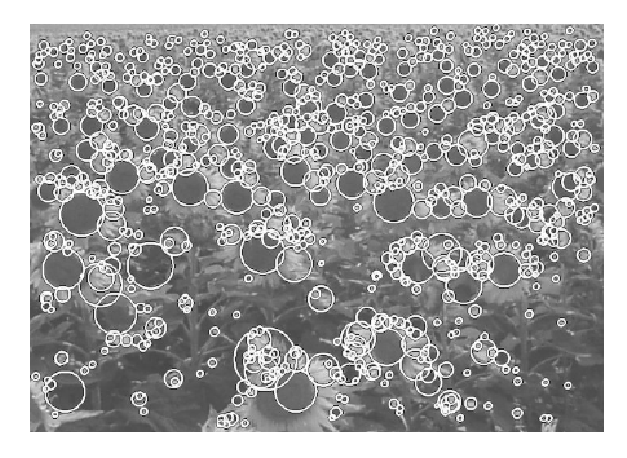
\includegraphics[scale=0.4]{./figs/pointsdetectedexampleimage}
    \caption[]{Puntos de interés detectados para un campo de girasoles. Este tipo de escenas muestra la naturalidad de las características obtenidas usando detectores basados en el Hessiano}
   \label{fig:pointsdetectedexampleimage}                %% Etiqueta para la figura entera
\end{figure}

\section{Descripción de los puntos de interés y Correspondencias}
Nuestro descriptor describe la distribución de intensidades en una vecindad del punto de interés, similar a la información del gradiente extraída por SIFT (24) y sus variantes. Se construye sobre la distribución de las respuestas de las wavelets Haar de primer orden en la dirección $x$ e $y$ en lugar de utilizar el gradiente, se utilizan las imágenes integrales para la velocidad y solo se usan 64 dimensiones. Esto reduce el tiempo de calculo y comparación de características y se ha demostrado que al mismo tiempo se incrementa la robustez. Además, se presenta un nuevo paso de indexación basado en el signo del Laplaciano, que incrementa no solo la robustez del descriptor, sino que también la velocidad de búsqueda de correspondencias (por un factor de 2 en el mejor de los caos). Nos referiremos a nuestro esquema de detector descriptor como SURF - Speeded up robust features.

El primer paso consiste en fijar una orientación posible basada en la información de una región circular alrededor del punto de interés. Luego, se construye una región cuadrada alineada con la orientación seleccionada y se extra el descriptor SURF de la misma. Finalmente, se busca la correspondencia de características entre imágenes. Estos tres pasos son explicados a continuación.

\subsection{Asignación de la orientación}
Con el objetivo de lograr invariancia a la rotación de la imagen, necesitamos identificar una orientación reproducible para el punto de interés. Para este propósito, primeros se calcula las respuestas de la Wavelet Haar en la dirección $x$ e $y$ en una vecindario circular de radio $6s$ alrededor del punto de interés, con $s$ la escala en la que se detectó el punto de interés. El paso de muestreo es dependiente de la escala y se elige que sea $s$. En consonancia con el resto, también el tamaño de las wavelets es dependiente de la escala y se establece a un longitud (lado) de $4s$. Por consiguiente, nuevamente se usan imágenes integrales para un filtrado rápido. Los filtros usados se pueden observar en la figura \ref{fig:haarwavelets}. Solo seis operaciones son necesarias para calcular las respuestas en la dirección $x$ o $y$ a cualquier escala.

\begin{figure}[tbhp]
   \centering
        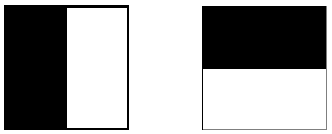
\includegraphics[scale=0.4]{./figs/haarwavelets}
    \caption[]{Filtros Wavelets Haar para calcular las respuestas en en la dirección de $x$ (izquierda) y $y$ (derecha). La parte negra tiene un valor de $-1$ y la blanca de $+1$.}
   \label{fig:haarwavelets}                %% Etiqueta para la figura entera
\end{figure}

Una vez que las respuestas wavelets han sido calculadas y ponderadas con una gaussiana ($\sigma = 2s$) centrada en el punto de interés, las respuestas son representadas como puntos en el espacio con la intensidad de la respuesta horizontal en la abscisa y la vertical a lo largo de la ordenada. La orientación dominante es estimada mediante el cálculo de la suma de todas las respuestas en una ventana deslizante orientada de tamaño $\pi/3$ como se observa en la figura \ref{fig:responsecalculate}. Las respuestas horizontales y verticales dentro de la ventana son sumadas. Las dos respuestas sumadas luego construyen un vector de orientación local. El vector más largo sobre todas las ventanas, define la orientación del punto de interés. El tamaño de la ventana deslizante es un parámetro que debe ser seleccionado cuidadosamente. Tamaños pequeños darán gradientes dominantes simples, tamaños grandes tienen a producir máximos en la longitud del vector que no son confiables. Ambos resultados, resultan en una orientación falsa del punto de interés.

\begin{figure}[tbhp]
   \centering
        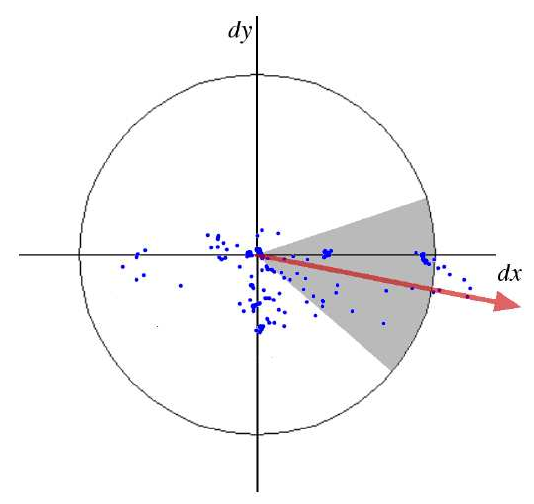
\includegraphics[scale=0.4]{./figs/responsecalculate}
    \caption[Asignación de la orientación]{Asignación de la orientación: una ventada orientada deslizante de tamaño $\frac{\pi}{3}$ detecta la orientación dominante de la respuesta de la wavelete haar ponderada con un gaussiano por cada punto en una vecindad circular alrededor del mismo.}
   \label{fig:responsecalculate}                %% Etiqueta para la figura entera
\end{figure}

Hay que hacer notar, que muchas aplicaciones no necesitan invarianza a la rotación. Experimentos usando la versión U-SURF para detección de objetos pueden ser encontradas en (3,4) (por ejemplo en robótica.). U-SURF es más rápido de calcular y puede aumentar la distintividad, mientras mantiene la robustez para rotaciones de $+/- 15\text{\ensuremath{\textdegree}}$

\subsection{Descriptor basado en la suma de las respuestas de la Wavelets Haar}
Para la extracción del descriptor, el primer paso consiste en construir una región cuadrada centrada alrededor del punto de interés y orientada a lo largo de la orientación seleccionada anteriormente. El tamaño de esta ventana es $20s$. Ejemplos de esas regiones cuadradas son ilustradas en la figura \ref{fig:squareregionsexample}

\begin{figure}[tbhp]
   \centering
        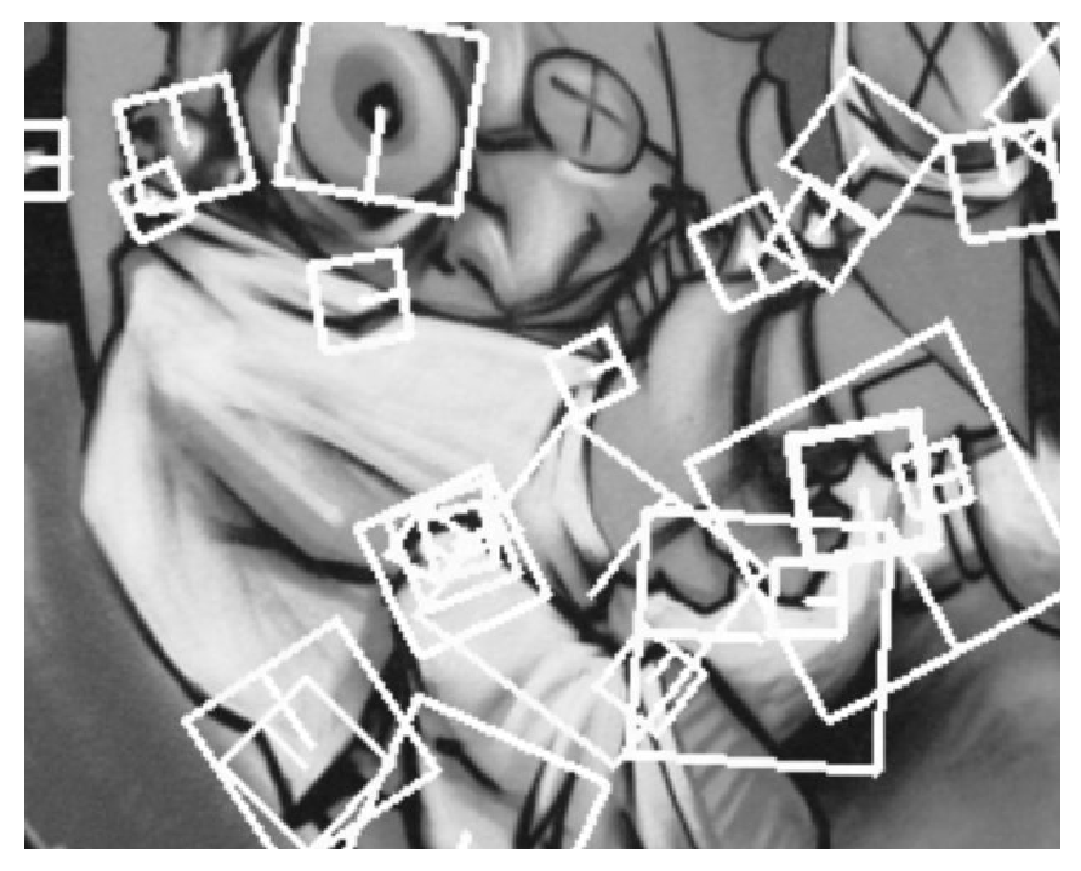
\includegraphics[scale=0.4]{./figs/squareregionsexample}
    \caption[]{Detalle de la escena graffiti mostrando el tamaño de las ventanas orientadas del descriptor a diferentes escalas}
   \label{fig:squareregionsexample}                %% Etiqueta para la figura entera
\end{figure}

La región es dividida regularmente en sub regiones cuadradas de 4x4. Esto preserva información espacial importante. Para cada sub región, se computan las respuestas de las wavelet haar cada 5x5 puntos de muestreo espaciados. Por razones de simplicidad, llamaremos $d_x$ a la respuesta de la wavelet haar en la dirección horizontal y $d_y$ en la dirección vertical (tamaño del filtro $2s$), véase la figura \ref{fig:haarwavelets} nuevamente. ``Horizontal'' y ``Vertical'' aquí es definido en relación a la orientación del punto de interés seleccionado (ver figura \ref{fig:subdivideregions})\footnote{Por razones de eficiencia, las Wavelets Haar son calculadas sobre una imagen sin rotar y las respuestas son interpoladas en lugar de rotar la imagen}. Para incrementar la robustez ante deformaciones geométricas y errores de localización, las respuestas $d_x$ y $d_y$ son primero ponderadas con un gassiano ($\sigma=3.3s$) centrado en el punto de interés.


\begin{figure}[tbhp]
   \centering
        \includegraphics[scale=0.4]{./figs/subdivideregions}
    \caption[]{Para construir el descriptor, una grilla cuadrática orientada con subregiones cuadradas de 4x4 se coloca sobre el punto de interés (izquierda). Para cada cuadrado, la respuesta de la wavelet es calculada. Las subdivisiones de 2x2 de cada cuadrado corresponde a los campos reales del descriptor. Estas son las sumas $dx$, $|dx|$, $dy$ y $|dy|$ calculadas relativas a la orientación de la grilla (derecha)}
   \label{fig:subdivideregions}                %% Etiqueta para la figura entera
\end{figure}

%%%%%%%%%%%%%%%%%%%%%%%%%%%%%%%%%%%%%%%%%begin: viene de parte 3 *************************************************************
\begin{figure}[tbhp]
   \centering
        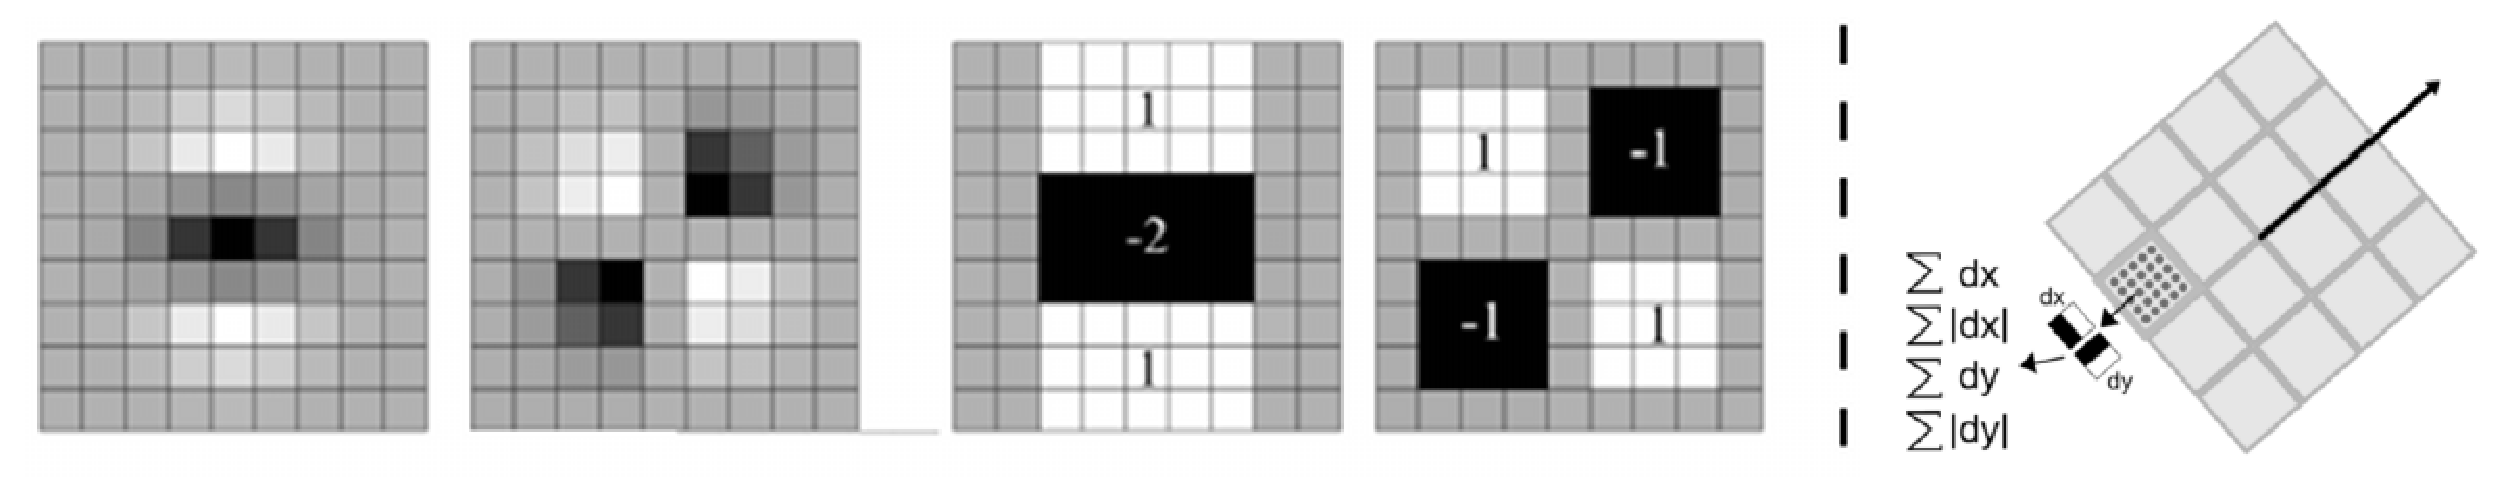
\includegraphics[scale=0.4]{../figs/left_boxfilters}
    \caption[]{Izquierda: Derivadas parciales gaussianas de segundo orden en la dirección Y y en la dirección XY, y sus aproximaciones usando filtros caja utilizados en SURF \ref{Bay:2008:SRF}. Derecha: el descriptor surf consiste en las respuestas de la wavelet Haar en una región de 4x4 alrededor del punto clave. \ref{Evans09noteson}}
   \label{fig:left_boxfilters}                %% Etiqueta para la figura entera
\end{figure}
%%%%%%%%%%%%%%%%%%%%%%%%%%%%%%%%%%%%%%%%%end: viene de parte 3 *************************************************************

Luego, las respuestas de la wavelet $d_x$ y $d_y$ son sumadas a lo largo de cada sub región y forman un primer conjunto de entradas del vector descriptor. Con el objetivo de brindar información a cerca de la polaridad de los cambios de intensidad, también se extrae la suma de los valores absolutos de las respuestas, $|dx|$ y $|dy|$. Por lo tanto, cada sub región tendrá un vector descriptor de 4 dimensiones $\mathbf{v}$ de su estructura subyacente de intensidad $\mathbf{v}=(\sum{d_x},\sum{d_y},\sum{|d_x|},\sum{|d_y|})$. Concatenando esto para todas las sub regiones de 4x4, esto resulta en un descriptor de longitud 64. Las repuestas wavelet son invariantes a un sesgo en la iluminación (offset). Invarianza al contraste (un factor de escala) es alcanzado mediante la conversión del descriptor a uno unitario.

\begin{figure}[tbhp]
   \centering
        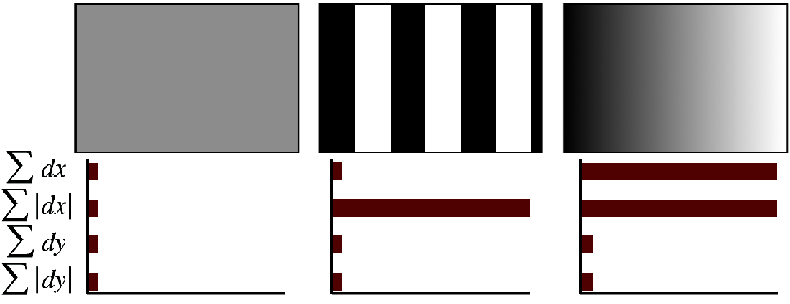
\includegraphics[scale=0.4]{./figs/descriptorresponses}
    \caption[]{Las entradas del descriptor de una sub región representan la naturaleza del patrón de intensidad subyacente. Izquierda: En el caso de una región homogénea, todos los valores son relativamente bajos. Medio: En presencia de frecuencias en la dirección de $x$, los valores de $\sum{|d_x|}$ son altos mientras los otros son bajos. Si la intensidad se incrementa gradualmente en la dirección $x$, ambos valores $\sum{d_x}$ y $\sum{|d_x|}$ son altos.}
   \label{fig:descriptorresponses}                %% Etiqueta para la figura entera
\end{figure}

La figura \ref{fig:descriptorresponses} muestra las propiedades del descriptor para tres patrones distintivos de intensidad diferente en una sub región. Uno puede imaginar una combinación de estos patrones de intensidad locales, resultando en un descriptor distintivo.

SURF es, hasta un cierto punto, conceptualmente similar a SIFT, en el sentido de que ambos se enfocan en la información de la distribución espacial del gradiente. Sin embargo, SURF supera a en la práctica a SIFT en todos los casos como se mostrará en la sección \ref{sec:seccion5}. Se cree que esto es debido al hecho de que SURF integra la información del gradiente en un sub parche, mientras que SIFT depende de las orientaciones de los gradientes individuales. Esto hace a SURF menos sensitivo al ruido, como se muestra en la figura \ref{fig:surflesssensitivetonoise}

\begin{figure}[tbhp]
   \centering
        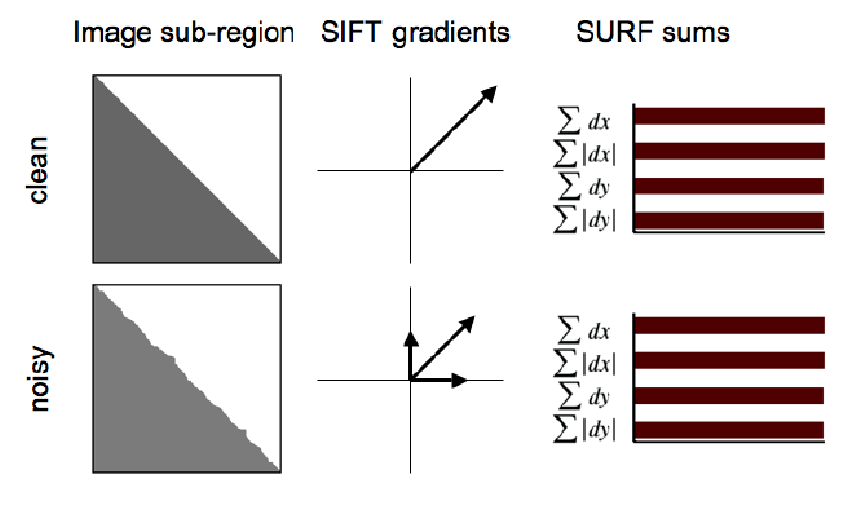
\includegraphics[scale=0.4]{./figs/surflesssensitivetonoise}
    \caption[]{Debido a la integración global del descriptor SURF, este se mantiene más robustos a varias perturbaciones en las imágenes que el descriptor de SIFT que opera más localmente.}
   \label{fig:surflesssensitivetonoise}                %% Etiqueta para la figura entera
\end{figure}
Con el fin de arribar a este descriptor SIFT, se ha experimentado con menos y más características wavelets, derivadas de segundo orden, wavelets de alto orden, PCA, valores medios, promedios, etc. De esta evaluación, el conjunto propuesto fue el que resultó con mejor rendimiento. Luego se variaron el número de puntos de muestras y sub regiones. La división de sub regiones en 4x4 dio los mejores resultados como se puede ver en la \ref{sec:seccion5}. Considerando subdivisiones más finas, pareció tener menos robustez y se incrementó el tiempo de correspondencias considerablemente. Por otro lado, un descriptor mas pequeño con subregiones de 4x4 (SURF-36) se desempeña un poco, pero permite correspondencias más rápidas y es aceptable ante otras comparaciones de la literatura. 

También hemos testeado otras versiones alternativas al descriptor SURF que añade un par de características similares (SURF-128). Se vuelven a utilizar las mismas cantidades que antes, pero ahora se dividen aún más. Las sumas de $d_x$ y $|d_x|$ son calculadas separadamente para $d_{y}<0$ y $d_{y}\geq0$. Similarmente, las sumas de $d_{y}$ y $|d_y|$ son divididas de acuerdo al signo de $d_{x}$, duplicando así el numero de características. El descriptor es más distintivo y no incrementa mucho el cálculo, pero es más lento de buscar correspondencias debido a su alta dimensionalidad.

\subsection{Indexación rápida para búsqueda de coincidencias}
Para la indexación rápida durante la etapa de coincidencias, el signo del laplaciano (por ejemplo la traza de la matriz hessiana) de los puntos de interés subyacentes es incluido. Comúnmente, los puntos de interés se hallan en regiones y puntos que difieren de su vecindad por su color o intensidad. El signo del laplaciano distingue regiones brillantes sobre fondos oscuros de la situación inversa. Esta característica está disponible sin un costo computacional extra debido a que ya ha sido calculada durante la fase de detección. En el paso de correspondencias, solo se comparan las características si tienen el mismo tipo de contraste, ver figura \ref{fig:contrastcomparation}. Por lo que esta información mínima permite correspondencias rápidas sin reducir la performance del descriptor. Esto también es una ventaja para los métodos más avanzados de indexación. Por ejemplo para k-d trees, esta información extra, define un hiper plano significativo para dividir los datos, opuesto a seleccionar un elemento aleatoriamente o usar estadísticas de características.

\begin{figure}[tbhp]
   \centering
        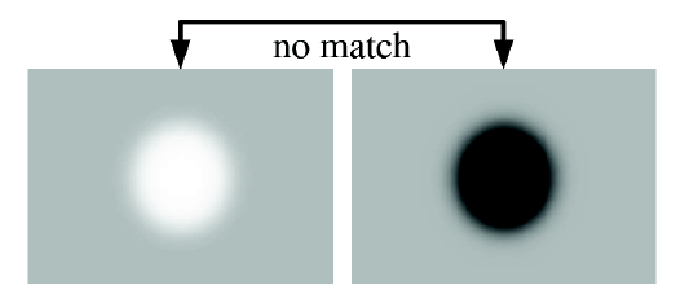
\includegraphics[scale=0.4]{./figs/notmatching}
    \caption[]{Si el contraste entre dos puntos de interés es diferente (oscuro sobre fondo claro versus claro sobre fondo oscuro), el candidato no es considerado como una coincidencia valiosa.)}
   \label{fig:contrastcomparation}
\end{figure}

% \section{Resultados}
% \label{sec:seccion5}
% Para un estudio comparativo con otros detectores y descriptores, nos referiremos a (4). SURF ya ha sido testeado en algunas aplicaciones reales. Para reconocimiento de objetos, su performance ha sido ilustrada en (3). Tomando esta aplicación para la registración de imágenes, nos enfocaremos en este artículo en el problema más difícil de calibración de la cámara y reconstrucción 3D, también en casos de wide-baseline.
% 
% \section{Conclusiones}
% Hemos presentado un detector y descriptor de puntos de interés rápido e invariante a escala y a rotación. La importante ganancia en velocidad se debe al uso de imágenes integrales, que reducen drásticamente el número de operaciones para convoluciones simples con filtros cajas, independientemente del tamaño de escala. La aproximación de Hessiano es comparable con los detectores de puntos de interés del estado del arte, resultado en casos aún mejor. Incluso sin realizar ningún tipo de optimización, un cálculo casi en tiempo real sin pérdida de rendimiento es posible, lo que representa una ventaja importante para muchas aplicaciones en linea de visión por computador.
% 
% El descriptor basado en la suma de las componentes de las Wavelets Haar, superan los métodos del estado de arte actual. La naturalidad de descripción del patrón intensidad subyacente de la imagen resulta ser más distintiva que los enfoques basados en histogramas. La simplicidad y el uso de las imágenes integrales, hacen al descriptor competitivo en términos de velocidad. Además, las estrategias de indexación basadas en el Laplaciano, hacen que las correspondencias sean más rápidas sin pérdidas en términos de performanse.

% \section{Análisis homográfico, proyecciones y transformaciones}

% \subsection{Correspondencia de imágenes}
% usando RANSAC}
% Cuando 2 cámaras observan la misma escena ven los mismos elementos pero bajo diferentes puntos de vista. Anteriormente en la sección \ref{subsub_calculo_matriz_fundamental} se ha estudiado el problema de la correspondencia entre puntos característicos. 
% En esta sección vamos a explotar las restricciones epipolares entre las dos vistas para lograr una correspondencia de características más fiable.
% A continuación, se expondrá como aprovechar las restricciones epipolares descriptas en la sección \ref{subsub_calculo_matriz_fundamental} para obtener una correspondencia de características más fiables, de tal forma de poder lograr una mejor estimación de la matriz fundamental.
% 
% Para lograr esta fiabilidad, sólo se aceptarán que los puntos característicos son coincidentes entre imágenes si los mismos caen sobre la línea epipolar correspondiente a cada uno de ellos. Para comprobar esta condición, nos encontramos con un nuevo problema: en primera instancia, la matriz fundamental debe ser conocida y como sabemos se necesitan buenas coincidencias para estimar bien esta matriz, de esta forma estamos en presencia de un problema mutuamente dependiente. Para poder resolverlo, se propone una solución en el que la matriz fundamental y un conjunto de buenas coincidencias son calculadas de forma conjunta.
% El objetivo es obtener un conjunto de buenas coincidencias entre las dos vistas. Por lo tanto, todas las correspondencias son validadas usando la restricción epipolar introducida en la sección anterior.

% A partir de los puntos característicos y sus descriptores, se procede a hallar la correspondencia para cada uno de los puntos %con la correspondencia mediante fuerza bruta. Si embargo, 
% ,buscándose %se buscan 
% las mejores dos coincidencias para cada característica basándose en una métrica de distancia, específicamente la euclídea.
% % lo cual es llevado a cabo mediante el knnMatch con $k==2$ 
% Este proceso, se lleva a cabo en ambas direcciones: por cada punto en la primer imagen, se buscan las dos mejores coincidencias en la segunda imagen, y viceversa. Luego, si la distancia medida es muy pequeña para la primer mejor coincidencia y muy grande para la segunda mejor coincidencia, se puede aceptar la primera como la mejor opción. Recíprocamente, si las dos mejores coincidencias son relativamente cercanas en distancia, se desechan ambas mediante un valor de umbral ya que puede haber un error si seleccionamos la primera o la segunda.
% % ya que puede haber un error si seleccionamos la primera o la segunda. 
% % De esta forma se logran eliminar gran cantidad de coincidencias ambiguas.
% 
% Si bien con los pasos descriptos anteriormente se logra reducir de forma considerable la cantidad de coincidencias ambiguas, si se está en presencia de una gran cantidad de buenas coincidencias \cite{citeulike:9456628}, un significante número de falsas coincidencias aún persiste, para lo cual se realiza un segundo filtrado para poder eliminar ambigüedades o coincidencias no validas como se expone a continuación.
% 
% Hasta el momento, se ha obtenido un conjunto de coincidencias de la primer imagen hacia la segunda y otro de la segunda hacia la primera. Así, se extraen las que son válidas en ambos conjuntos mediante un esquema de coincidencias simétrico: un par de coincidencias es aceptada como válida si ambos puntos son la mejor característica de coincidencia en cada una de las imágenes.% imágenes.
% 
% % En este punto se tiene un conjunto de coincidencias relativamente bueno, uno para la primer imagen hacia la segunda y otro de la segunda imagen hacia la primera. De estos conjuntos, se extraen las coincidencias que son validas en ambos conjuntos. Este es el esquema de coincidencias simétrico que establece que para que un par de coincidencias sean aceptadas como validas, ambos puntos deben ser la mejor característica que coincida en la otra.
% 
% Finalmente, se agrega otro paso de filtrado el cual consiste en usar la matriz fundamental con el objetivo de descartar coincidencias que no cumplen con la restricción epipolar. Este test está basado en el método RANSAC (Muestras aleatorias consensuadas, del inglés: Random Sample Consensus) \cite{Hartley2004, Fischler:1981:RSC:358669.358692, BMVC.23.81, Chum-PhD-TR-2005-19}, que puede calcular la matriz fundamental aún cuando valores atípicos están presentes en los conjuntos de datos.
% % de coincidencias.
% Debemos notar que los diferentes pasos para eliminar ambigüedades y coincidencias invalidas, son llevados a cabo con el objetivo de lograr un conjunto de datos fiables que es necesario para lograr una buena estimación de la matriz. En caso de no hacerlo, posiblemente se estaría en presencia de un resultado no deseado y poco fiable.

% \subsubsection{RANSAC}
% El objetivo del algoritmo RANSAC, es estimar una entidad matemática dada desde un conjunto de datos que contiene valores atípicos o incorrectos. Se basa en la idea de seleccionar puntos del conjunto de forma aleatoria llevando a cabo la estimación sólo con este conjunto de datos. El número de puntos seleccionados debe ser el mínimo requerido para estimar la entidad matemática en cuestión, así en el caso de la matriz fundamental, ocho pares de coincidencias resulta ser la cantidad necesaria (podrían ser siete, pero tomar 8 produce un algoritmo lineal que es más rápido de resolver). Una vez que la matriz fundamental es estimada con estas ocho coincidencias aleatorias, todas las demás coincidencias en el conjunto son probadas con la restricción epipolar que se deriva de esta matriz. Todas las coincidencias que cumplen esta restricción, es decir, coincidencias para las cuales la característica correspondiente se encuentra a una distancia cercana de la línea epipolar, son identificadas para formar parte del ``conjunto soporte'' de la matriz fundamental calculada.
% 
% La idea central detrás del algoritmo RANSAC es que cuanto mayor sea el ``conjunto soporte'', mayor será la probabilidad de que la matriz calculada sea la correcta, de manera que si una (o más) de las coincidencias aleatorias seleccionadas son malas coincidencias, la matriz fundamental calculada seguramente será una mala estimación y por lo tanto, se espera que el conjunto soporte sea menor. Este proceso es repetido varias veces y finalmente se toma como más probable a la matriz con el soporte más grande.
% 
% Resumiendo, el objetivo es tomar varias veces ocho coincidencias de forma aleatoria, de manera que eventualmente seleccionemos ocho buenas coincidencias que nos provean de un conjunto soporte grande. Dependiendo de la cantidad de falsas coincidencias que haya en todo el conjunto de datos, la probabilidad de seleccionar un conjunto de ocho coincidencias correctas diferirá. Sin embargo, sabemos que cuanto más selecciones hagamos, mayor será la confianza en encontrar por lo menos un conjunto de buenas coincidencias.

%  Más precisamente, si asumimos que el conjunto de coincidencias posee $b\%$ buenas coincidencias, luego, la probabilidad de que la selección contenga al menos una coincidencia con un valor atípico es $(1-b8)$. Si hacemos $k$ selecciones, la probabilidad $c$ de tener un conjunto de datos aleatorio que contenga solamente buenas coincidencias es $c=1-(1-8b)k$. Esta es la confianza de probabilidad $c$ y queremos que esta probabilidad sea lo más alta posible ya que necesitamos por lo menos un conjunto de buenas coincidencias para poder obtener la matriz fundamental correcta. Por lo tanto, cuanto se ejecuta el algoritmo RANSAC, uno necesita determinar el número de selecciones $k$ que necesita usar, con el objetivo de obtener el mejor nivel de confianza.

% Cuando se usa la función $cv::findFundamentalMat$ con RANSAC, dos parámetros extras son provistos. El primero es el nivel de confianza que determina el número de iteraciones a realizar. El segundo es la distancia máxima a la linea epipolar para que el punto sea considerado como valido.

% Cuanto mayor sea la cantidad de coincidencias válidas en el conjunto inicial, mayor es la probabilidad de que obtengamos la matriz fundamental correcta con el algoritmo RANSAC, es por esto que antes de buscar la matriz fundamental se aplican todos los pasos anteriormente descriptos de manera de filtrar las posibles coincidencias espurias.

% La mayor cantidad de macheos buenos que tenga en el conjunto inicial, aumenta las probabilidades de que Ransac de la matriz fundamental correcta. Por eso se aplican varios filtros a los match antes de llamar a la función para buscar la matriz fundamental.

% \subsubsection{Calculando la homografía entre dos imágenes}

%%%%%%%%%%%%%%%%%%%%%%%%%%%%%%%%%%%%%%%%%%%%%%%%%%%%%%%%%%%%%%%%%%%%%%%%%%%%%%%%%%%%%%%%%%%%


% 
% 
% 
% Como se explicó anteriormente, una vez que sea logrado obtener la homografía, todos los puntos en una vista pueden ser convertidos a la segunda vista usando la relación \eqref{eq:eq_ecuacion_rel_homography_ptos}.
% % una vez que la homografía es calculada, es posible mediante la misma transferir los puntos de una imagen en una vista al punto de vista de otra.
% Cuando dos vistas estan relacionadas por la homografía, se hace posible determinar en que lugar un punto de la escena en una imagen puede ser encontrado en la otra. Esta propiedad se hace interesante para puntos que caen fuera de los bordes de la imagen. De hecho, desde que la segunda vista muestra una porción d e la escena que no es visible en la primera imagen, se puede usar la homografía para expandir la imagen mediante la lectura del valor de color de los pixeles adicionales. Así es como se puede crear una nueva imagen que es una expansión de la segunda imagen en la que las columnas extras son añadidas a la derecha.
% La homografía calculada por $cvFindHomography$ es aquella que mapea los puntos de la primer imagen a puntos en la segunda imagen.

% Lo que se necesita para transferir puntos de una imagen a otra es la homografía inversa. Esto es exactamente lo que hace la función cvWarpPerspective por defecto, usa la inversa de la homografía proporcionada como entrada para obtener el valor del color de cada punto de la imagen de salida. Cuando un pixel de salida es transferido a un punto fuera de la imagen de entrada, se asigna el valor 0 (negro) a ese píxel.
% Una homografía también existe entre dos vistas de un plano. Esto puede ser demostrado mirando nuevamente las ecuaciones de proyección de la cámara, como se hizo en el caso de rotación pura. Cuando un plano es observado, podemos, sin perder generalidad, establecer el frame de referencia del plano de tal forma que todos sus puntos tengan la coordenada $Z=0$. Esto cancela una de las columnas de la matriz de proyección de $3x4$ resultando en una matriz de $3x3$: la homografía. Esto significa que por ejemplo, si se tienen imágenes de diferentes puntos de vistas de una fachada plana de un edificio, se puede calcular la homografía entre las imágenes y construir un largo mosaico de la fachada ensamblando las imágenes de la forma que se describió anteriormente. 
% 
% De esta forma, se puede utilizar una imagen que se quiera sobre imponer aplicándole la inversa de la homografía calculada anteriormente de forma de obtener los puntos correspondientes donde debería dibujarse en el flujo de video y así lograr el efecto de sobre imponer el objeto virtual en la realidad. 
% Existe una función provista por la librería OpenCV que aplica una transformación perspectiva a una imagen denominada cvWarpPerspective()\footnote{\url{http://opencv.willowgarage.com/documentation/cpp/imgproc_geometric_image_transformations.html\#cv-warpperspective}} y que es la usada para llevar a cabo esta tarea.
% Cabe aclarar que un mínimo de cuatro correspondencia es requerido para calcular la homografía.
% La función cvGetPerspectiveTransform permite una transformación de los 4 puntos correspondientes a calcular.
%%%%%%%%%%%%%%%%%%%%%%%%%%%%%%%%%%%%%%%%%%%%%%%%%%%%%%%%%%%%%%%%%%%%%%%%%%%%%%%%%%%%%%%%%%%%%%%%%%%%%%%%%%%%